It is known that the cost of the pod infrastructure is highly coupled with the
Mach number at which the vehicle travels. In order to obey the choking constraint,
higher Mach numbers will necessitate a larger tube to prevent the flow around
the pod from accelerating to the speed of sound. This increases the material
cost of the tube and the energy required to pump down the tube. In this analysis,
the full system model will be run for a range of Mach numbers.
For each Mach number, the area of the tube is recorded along with total energy cost.
In this analysis, the leakage rate is assumed to be a constant mass flow on the order 1 kg/s.
This value should be sufficient for illustrating the trend of energy
consumption as a function of Mach number. Different values of leakage rate will
not significantly alter the trend, but will instead directly scale the amount
of energy used by the vacuum system in a steady state condition.
\begin{figure}
	\centering
	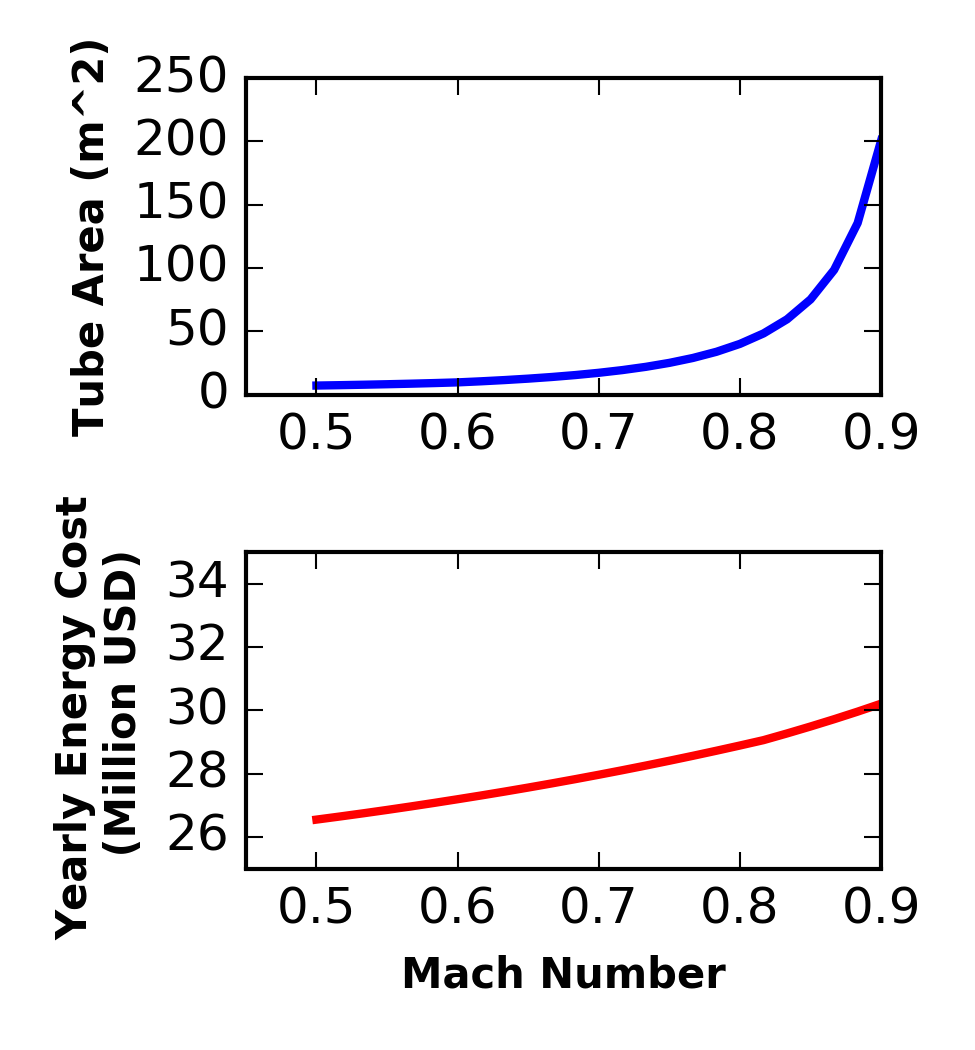
\includegraphics{../../images/graphs/mach_trades/pressure_vs_mach.png}
	\caption{Tube Area and Yearly Energy Cost vs. Mach Number}
	\label{fig:tube_area_cost_vs_mach}
\end{figure}
\Cref{fig:tube_area_cost_vs_mach} Indicates the how tube area and energy
consumption change over a range of Mach numbers. As is indicated in previous research,
tube area begins to increase rapidly around Mach .8 \cite{Chin}.
Beyond this Mach number, small increases in Mach number result in a large
increase in tube area, which will have a large impact on capital cost and pump
down energy of the system. Conversely, \cref{fig:tube_area_cost_vs_mach}
indicates that there is very little marginal material cost required to increase
Mach number. The increase in energy consumption is much more modest; however,
the mild increase in energy cost is dominated by the increase in material cost
for higher Mach numbers. Based on these results, it is estimated that any
system level optimization of cost with respect to Mach number will result in a
Mach number near .8. For this reason, a Mach number of .8 will be used in
subsequent analyses to obtain reasonable evaluations of design trades and system behavior.
